\documentclass[a4paper,10pt]{article}
\usepackage[lmargin=2.0cm, rmargin=1.0cm,tmargin=3.5cm,bmargin=1.5cm]{geometry}
\usepackage{color,graphics}
\usepackage[export]{adjustbox}
\usepackage{lipsum}
\usepackage{multirow}
\usepackage{graphicx}
\usepackage{xfrac}
%\usepackage{lstlisting}
\usepackage{listings}
\usepackage[scaled=0.75]{helvet}
\usepackage{amsmath}
\usepackage[options ]{algorithm2e}
\usepackage{amsfonts}
\usepackage{verbatim}
\usepackage{algpseudocode}
\definecolor{dkgreen}{rgb}{0,0.6,0}
\definecolor{gray}{rgb}{0.5,0.5,0.5}
\definecolor{mauve}{rgb}{0.58,0,0.82}
\makeatletter
\newcommand{\algrule}[1][.2pt]{\par\vskip.5\baselineskip\hrule height #1\par\vskip.5\baselineskip}
\makeatother
\begin{document}
\setcounter{secnumdepth}{-1} 
\begin{center}
\textbf{\LARGE  Implementation of Support Vector Machine Classification using R package - Caret for Iris Dataset.}
\end{center}

\raggedright Expt No: 7 (a) \hfill \raggedleft May 2,2019 \\ 

\raggedright Author: Subalakshmi Shanthosi S (186001008) \par 

\noindent\makebox[\linewidth]{\rule{\textwidth}{1pt}} 

\section{Aim}
Implementation of Support Vector Machine(SVM) using R package- Classification and Regression Training(CARET) for Iris dataset classification.

\section{Description}
\begin{enumerate}
	\item Support Vector Machine:
	\begin{itemize}
		\item Support Vector Machine is a Supervised Learning Model.
		\item SVM can be applied for both classification and regression algorithms but predominantly used for classification problems.	 
		\item Support Vector Algorithm Working:
		\begin{itemize}
		 \item Input : Data points from the dataset (iris).
		 \item Output : Hyperplane - The line which best separates the tags.
		 \item Careful choice of Kernal function which decides the accuracy of the model.	
		\end{itemize}
	    \item Advantages of using SVM for classification:
	    \begin{itemize}
	    	\item High Dimensionality.
	    	\item Memory Efficiency.
	    	\item Versatility.	
	    \end{itemize}
       \item Disadvantages of using SVM:
       \begin{itemize}
       	\item Kernel Parameters Selection : SVM shows poor performance on higher dimensional data.
       	\item Non-Probabilistic : Effectiveness is less evident as the algorithm places few data points above and below the decision boundry which might lead to misclassification if the between class varients among points is less.
       \end{itemize}	
	\end{itemize}
    \item Classification hyperplane based on the data point's distribution is presented below:
     \begin{figure}[h]
    	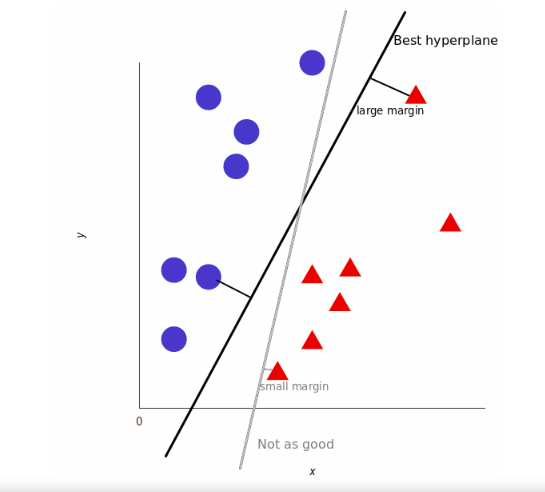
\includegraphics[scale=0.30,center]{svmClassification.png}
    	\caption{SVM Linear Model.}
    	\label{fig:1}
    \end{figure}
    \begin{figure}[h]
    	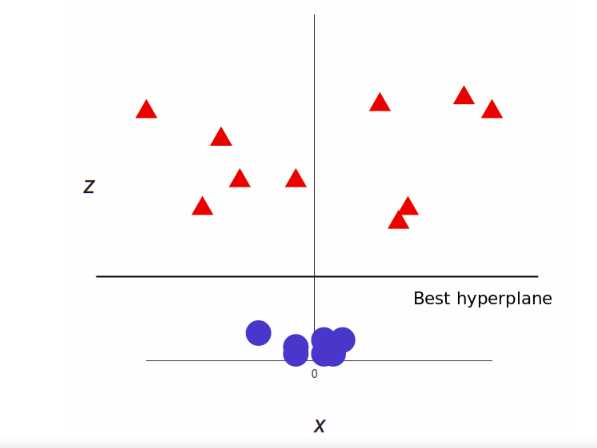
\includegraphics[scale=0.30,center]{svmNonLinearData.png}
    	\caption{SVM Non Linear model by 3-D projection.}
    	\label{fig:2}
    \end{figure}
    
\end{enumerate}

\pagebreak
\section{Tools and Packages}
\begin{enumerate}
	\item Tools
	\begin{itemize}
		\item RStudio.
		\item R Version 1.1.463
	\end{itemize}
	\item Support Vector Machine and Visualisation Packages
	\begin{itemize}
		\item caret
		\item ggplot2 (Visualisation)
		\item GGally (Visualisation)
	\end{itemize}				
\end{enumerate}

\section{Dataset Description - Iris}
\begin{itemize}
	\item This famous (Fisher's or Anderson's) iris data set gives the measurements in centimeters of the variables sepal length and width and petal length and width, respectively, for 50 flowers from each of 3 species of iris. The species are Iris setosa, versicolor, and virginica.
	
	\item Iris is a data frame with :
	\begin{itemize}
		\item 150 cases (rows).
		\item 5 features/variables(columns):
		\begin{itemize}
			\item Sepal Length.
			\item Sepal Width.
			\item Petal Length.
			\item Petal Width.
			\item Species.
		\end{itemize}
	   \item  Iris \textit{setosa} is linearly separable from \textit{ Iris versicolor and virginica}
	\end{itemize} 	
\end{itemize}
\section{Procedure}

\begin{enumerate}
	\item Split the data set as:
	\begin{itemize}
		\item Training dataset.
		\item Testing dataset.
	\end{itemize}
	\item Exploratory data Visualisation : To decide on the model to fit for a better precision in classification.
	\item Feature Scaling and Model Fitting.
	\item Calculate prediction and evaluate the SVM model/kernal accuracy.
	\item Display the confusion matrix.
\end{enumerate}	

\section{Support Vector Machine}

\begin{itemize}
	\item Support Vector Machine is a machine learning algorithm which:
	\begin{enumerate}
		\item Solves classification problems.
		\item Uses flexible representation of decision boundary.
		\item Implements automatic complexity control to reduce overfitting.
		\item A single global minimum which can be found in polynomial
		time.
	\end{enumerate}
    \item  Pseudocode :
    
    \begin{algorithm}
    	\caption{The Support Vector Algorithm}
    	\algrule
    	\begin{itemize}
    		\Statex \textbullet~\textbf{Initialisation:}
    		\begin{itemize}
    			\item For the specified kernel, and kernel parameters, compute the kernel of distances between the datapoints.
    			\item The main work here is the computation K=XX\textsuperscript{T}.
    			\item For the linear kernel, return K, for the polynomial of degree d return $\frac{1}{\sigma K \textsuperscript{d}}$.
    		    \item For the RBF kernel, compute K = $\exp(-\frac{(x-x\textsuperscript{'})^2}{2\sigma\textsuperscript{2}})$.
    	\end{itemize}
    	\Statex \textbullet~\textbf{Training}
    		\begin{itemize}
    			\item Assemble the constraint set as matrices to solve:
    			\begin{equation}
    				min\textsubscript{x} \frac{1}{2}x\textsuperscript{T}t\textsubscript{i}t\textsubscript{j}K\textsubscript{x}+q\textsuperscript{T}x.
    			\end{equation}
    			subject to 
    			$G\textsubscript{x}<=h$
    			\linebreak
    			$A\textsubscript{x}=b$
    			\item Pass these matrices to the solver.
    			\item Identify the support vectors as those that are within some specified distance of the closest point and dispose of the rest of the training data.
    			\item Calculate b\textsuperscript{*} using equation:
    			\begin{equation}
    				b\textsuperscript{*}=\frac{1}{N\textsubscript{s}}\sum_{all support vectors}(t\textsubscript{j}-\sum_{i=1}^{n}\lambda\textsubscript{i}t\textsubscript{i}x\textsubscript{i}\textsuperscript{T}x\textsubscript{j}) .
    			\end{equation}
    		\end{itemize} 
    	    \Statex \textbullet~\textbf{ Classification}
    	    \begin{itemize}
    	    	\item For the given test data \textbf{z}, Use the support vector to classify the data for the relevant kernal by : 
    	    	\begin{itemize}
    	    		\item Compute the inner product of the test data and the support vectors.
    	    		\item Perform the classification as:
    	    		\begin{equation}
    	    			\sum_{i=1}^{n}\lambda\textsubscript{i}t\textsubscript{i}K(x\textsubscript{i},z)+b\textsuperscript{*}.
    	    		\end{equation}
    	    		returning -
    	    		\linebreak
    	    		The label (Hard Classification)
    	    		\linebreak
    	    		The value(Soft Classification)
    	    	\end{itemize}
    	    \end{itemize}
    	\end{itemize}
\algrule
    \end{algorithm}

\end{itemize}

\newpage
\section{Confusion Matrix}
\begin{itemize}
\item A confusion matrix is a table that can be generated for a classifier on a Data Set 

\textbf{True Positives(TP)-} These are the cases where the predicted and actual both are yes.
\linebreak
\textbf{True Negatives(TN)-} These are the cases where the predicted value is no and actual value is yes.
\linebreak
\textbf{False Positive(FP)-} These are the cases where the predicted value is yes and actual value is no.
\linebreak
\textbf{False Negative(FN)-} These are the cases where prediction is no and actual value is no.
\end{itemize}

\section{Coding}

\lstinputlisting{svmIris.r}
\section{Output} 
\verbatiminput{svmOutput.txt}

\fbox{\begin{minipage}{35em}
		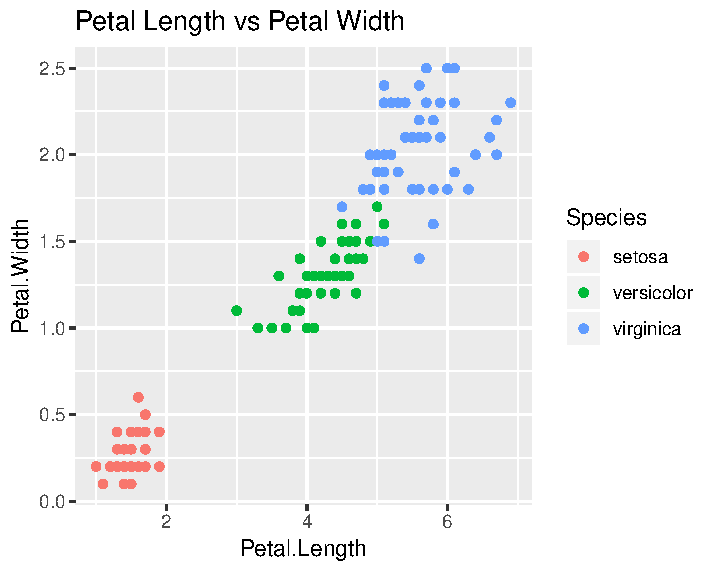
\includegraphics[page=1,scale=0.7]{svm.pdf}
	\end{minipage}}

\section{Result}
Thus the implementation of Support Vector machine is executed successfully using R program.


\end{document}